\documentclass{sig-alternate-05-2015}


\begin{document}

% Copyright
\setcopyright{acmcopyright}
%\setcopyright{acmlicensed}
%\setcopyright{rightsretained}
%\setcopyright{usgov}
%\setcopyright{usgovmixed}
%\setcopyright{cagov}
%\setcopyright{cagovmixed}

% DOI
\doi{xx.xxx/xxx_x}

% ISBN
\isbn{xxx-xxxx-xx-xxx/xx/xx}

%Conference
\conferenceinfo{}{}

\acmPrice{}

%
% --- Author Metadata here ---

%\CopyrightYear{2007} % Allows default copyright year (20XX) to be over-ridden - IF NEED BE.
%\crdata{0-12345-67-8/90/01}  % Allows default copyright data (0-89791-88-6/97/05) to be over-ridden - IF NEED BE.
% --- End of Author Metadata ---

\title{A System for Simulation-based, Emergent, Interactive Narrative Generation}
\subtitle{\large\textrm{INTERIM REPORT\\ (16/11/2018)}}
%
% You need the command \numberofauthors to handle the 'placement
% and alignment' of the authors beneath the title.
%
% For aesthetic reasons, we recommend 'three authors at a time'
% i.e. three 'name/affiliation blocks' be placed beneath the title.
%
% NOTE: You are NOT restricted in how many 'rows' of
% "name/affiliations" may appear. We just ask that you restrict
% the number of 'columns' to three.
%
% Because of the available 'opening page real-estate'
% we ask you to refrain from putting more than six authors
% (two rows with three columns) beneath the article title.
% More than six makes the first-page appear very cluttered indeed.
%
% Use the \alignauthor commands to handle the names
% and affiliations for an 'aesthetic maximum' of six authors.
% Add names, affiliations, addresses for
% the seventh etc. author(s) as the argument for the
% \additionalauthors command.
% These 'additional authors' will be output/set for you
% without further effort on your part as the last section in
% the body of your article BEFORE References or any Appendices.

\numberofauthors{2} %  in this sample file, there are a *total*
% of EIGHT authors. SIX appear on the 'first-page' (for formatting
% reasons) and the remaining two appear in the \additionalauthors section.
%
\author{
% You can go ahead and credit any number of authors here,
% e.g. one 'row of three' or two rows (consisting of one row of three
% and a second row of one, two or three).
%
% The command \alignauthor (no curly braces needed) should
% precede each author name, affiliation/snail-mail address and
% e-mail address. Additionally, tag each line of
% affiliation/address with \affaddr, and tag the
% e-mail address with \email.
%
% 1st. author
\alignauthor
Oliver Mitchell\\
       \affaddr{University of Nottingham}\\
       \email{psyom1@nottingham.ac.uk}
% 2nd. author
\alignauthor
Peter Blanchfield\\
       \affaddr{University of Nottingham}\\
       \email{peter.blanchfield@nottingham.ac.uk}
}
% There's nothing stopping you putting the seventh, eighth, etc.
% author on the opening page (as the 'third row') but we ask,
% for aesthetic reasons that you place these 'additional authors'
% in the \additional authors block, viz.

\maketitle
\begin{abstract}
Recent research in the field of interactive storytelling (IS) has focused on the advantages of ``emergent narratives'' (ENs). With this approach, the storyline `emerges' at run-time from the interactions between author-programmed autonomous agents and the player. The benefit is a non-linear narrative, allowing for greater player interactivity. However, ENs are unpredictable at authoring time, removing control over the plot's structure. The struggle to balance the author's control over the narrative, whilst simulatenously allowing the player to influence the story's direction, has been dubbed the ``Narrative Paradox''. We discuss the design and implementation of a new hybrid emergent storytelling system for creating unscripted narratives which aims to integrate the successful components of existing approaches, including an appraisal-driven agent architecture extended to model autobiographical memory, and a ``virtual director'' which maintains storyworld knowledge and uses a novel metaheuristic genetic algorithm to generate suitable global events for agents to appraise and respond to. An evaluation of the system's effectiveness (based on comparative user-testing) is discussed with a particular regard to player `immersion' and the believability of the generated narrative.
\end{abstract}

% We no longer use \terms command
%\terms{Theory}

\keywords{interactive storytelling; games; 
autonomous virtual agents; emergent narratives}

\section{Background}

\subsection{Defining Interactive Storytelling}

Interactive storytelling is a unique form of narrative design seen in digital entertainment mediums where no pre-determined storyline exists. Instead, the user can change the story and influence the characters themselves. Bostan and Marsh define interactive storytelling as an approach to computer game narrative design where ``real-time feedback collected from the players is used by the game engine to continuously modify the content as it is being delivered.'' [1]. The key aspect of interactive storytelling is that the player is an active participant and their in-game actions have a direct effect on the narrative that is told. This differs from traditional computer game narratives which typically consist of an unchanging linear story with a pre-defined outcome.

\subsection{Problems with the Integration of Interactivity into Game Narratives}

In most computer games, attempts at complex, dynamic storylines are usually ``confined to simple branching tree structures'' [3]. Furthermore, as the scope of games increases and development effort is focused on assets such as textures, 3D-modelling and other gameplay content, a greater number of narrative possibilities arise. However, the ``static nature of these [tree] structures affects the range of options covered [and] reduces the framework for player interaction''. Louchart et al. suggest ``the integration of interactivity into game narratives requires a rethinking of the design process'' [3]. This is because story trees have to expand exponentially with the inclusion of more narrative elements (such as additional characters added to the game) or risk remaining so simple and rigid that the player's immersion in the game world is threatened.

In short, with a greater amount of gameplay content comes infeasible exponential growth in the number of branches of a narrative tree structure. When there are too many branches, developers are forced to simplify the story, resulting in less player interactivity.

\subsection{The Narrative Paradox}

It is common for narrative design in computer games to follow a plot-based approach. Louchart and Aylett recognised that the ``authoring of interactive narrative presents the paradox that ... the author requires control over the unfolding narrative whilst ... the user expects freedom over their decisions.'' [3][4]. These two goals clearly conflict. The greater the level of interactivity provided to the player, the less control the author has over the story's events. Equally, the more control the author has over the story, the less room there is for the player to interact with characters and change the course of the narrative. This concept has been dubbed the ``Narrative Paradox'' [5]. Louchart and Aylett suggest that a solution to this paradox should divert from the branching plot-based approaches implemented in current computer games.

\subsection{Emergent Narrative}

Aylett proposed Emergent Narratives (EN) as an alternative. ENs are an approach to interactive story design where, instead of a static authored plot, the ``narrative weight of the application is shared by authors and players.'' [3][5][6]. This is typically achieved by simulating a virtual world, including characters with different behaviours, personalities and goals created by the author. The storyline then `emerges' at run-time from the interactions between these autonomous agents and the player [2]. The advantage of an EN approach is a non-linear narrative \textbf{(Figure 1)} that allows for a greater level of player interactivity. Despite this, ENs are unpredictable at authoring time. Kriegel and Aylett explain how authors are forced to ``let go of specific story lines altogether and ... focus on creating the elements from which the story will emerge.'' [7]. ENs work as a sort of `sandbox' where the author defines the limits of the story world and creates the characters and behaviours that fill it, then leaves the simulation to create its own story, providing no further input during run-time. As a result, authors of ENs will find it very difficult to ensure the story includes specific plot points.\\

\newline ENs benefit from having no rigid structure to their story because there is no branching tree restricting the range of storylines. This solves the problem of infeasible exponential growth because there are no branches to manage and the storyline emerges on its own. This allows for a potentially inumerable amount of emergent storylines (should the simulation be complex enough).

Despite this, a disadvantage of emergent narratives are their reliance on well implemented virtual agents and their control logic. If the AI controlling each agent is too simple, then the story is unlikely to be complex enough to satisfy the player. Or, if the AI has too limited a set of possible responses to stimuli in its environment, the player may see the same storylines again and again, threatening the narrative's believability.

\begin{figure}
\centering
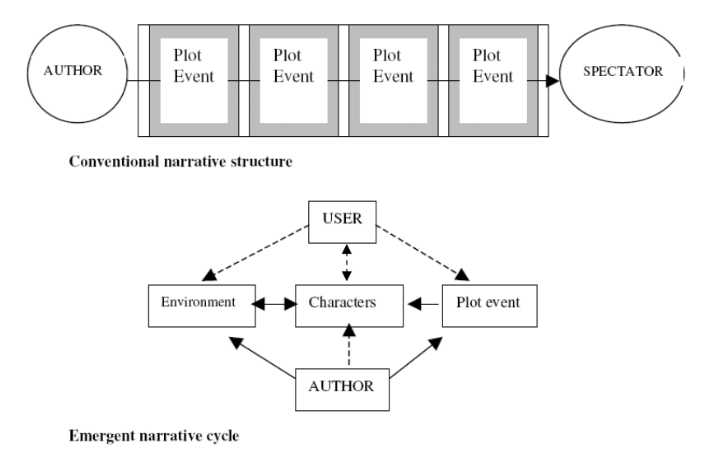
\includegraphics[scale=0.3]{Images/PlotVsEmergent.png}
\caption{Diagram showing the difference in structure between convential plot-based narratives and interactive emergent narratives. The former is static and sequential, whereas the latter is simulation-based and reacts to player interaction. [3]}
\label{fig:PlotVsEmergent}
\end{figure}

\subsection{Motivation}

\noindent The motivation for this project is to develop a new approach to interactive storytelling which utilises and combines components of successful, existing emergent narrative systems in order to generate compelling stories and give players a greater sense of agency. It is also crucial to provide adequate control of the narrative to authors. This will be achieved through a suite of story creation tools which allow authors to define characters personalites, goals and actions in detail. This paper focuses on simulation-based approaches which exploit the usefulness of emergent narratives and omit the restrictions of plot-based designs.

\section{Related Work}
\subsection{History of Digital Storytelling}
\subsubsection{Early approaches}
Since the 1970s, there have been many digital storytelling systems developed both in research and for commercial games. Early examples of story generation include \textit{Novel Writer}, a system that generated 2000+ word murder mystery stories that emerged from the actions simulated by each character [8], and \textit{TaleSpin}, a complex system that modelled rational behaviour for each character, including the production of personal goals that each agent could attempt to achieve autonomously through the creation of its own plan; a series of actions it may take [9]. \textit{Virtual Storyteller} was another system that, despite a lack of interaction, created stories via the actions and cooperation of intelligent agents. In this system plots are not pre-defined but created by the actions of the agents alongside a ``virtual director''; a seperate agent that maintains general story-world knowledge about the plot structure. It uses this to judge whether a character's intended actions fit into the narrative in order to produce a ``good'' plot; a believable and generally compelling story. Consequently, unlike the full-autonomy displayed in \textit{TaleSpin}, the agents in \textit{Virtual Storyteller} can only be considered semi-autonomous because they are consistently guided in their actions to create a well-structured plot [10]. Note that other systems explored in this paper utilise a similar ``virtual director'' type agent. However, those systems use such a device to manage and facilitate the creation of new storylines, \textbf{not} to perform global action control for individual agents, as seen in \textit{Virtual Storyteller}.\\

\newline Despite producing compelling emergent narratives, none of these systems can be considered examples of interactive storytelling because they do not allow a user to change the path of the story at run-time (\textit{Novel Writer} and \textit{TaleSpin} only accepted user input for the initial storyworld state and \textit{Virtual Storyteller} allows for no user input whatsoever, relying solely on its encapsulated virtual director to direct the plot).\\

\subsubsection{Towards Emergent Narratives}

\noindent Following these initial approaches came a greater focus on emergent storytelling and a move towards non-branching, character-focused systems. Aylett first coined the term ``emergent narrative'' in 1999 when discussing the narrative issues arising from placing children's TV characters in a virtual environment where they and the user had a joint spacial existence [6]. The original television narrative was wholly pre-scripted and viewed passively by the audience from camera positions determined by the creators. This strategy is unsuitable for use in a virtual environment where the user is transformed from a spectator to a potential participant. Aylett argues that a pre-determined narrative means the role of the user must also be pre-determined. Therefore, relaxing this constraint allows the user to be more freely involved [6].

The solution is to build the narrative from the bottom-up through the interactions of the characters. Many groups have looked at producing emergent narratives by treating characters as virtual actors [23][24]. In such a scenario, the focus of the user is moved from a participant to a director, where they're able to construct narratives involving virtual actors and themselves. This has been compared to the playtime of young children where they switch repeatedly between particpant and director in order to control the direction of their roleplay [6].

\subsection{Existing Emergent Narrative Systems}

\subsubsection{Automated Planning with HTNs}

Cavazza et al. produced a prototype character-based system which focused on defining the possible actions of individual characters in hierarchical task networks (HTN) in order to create automated plans and achieve character desired goals [11]. Characters act autonomously, executing available actions in their HTN in order to reach their goal, similar to the \textit{TaleSpin} system's character plans [9].  Each action is categorised and used to determine other characters' reactions (e.g. characters will react negatively to ``rude'' actions). The system also includes ``mood values'' for each character which can affect other characters' plans. Because the system allows for emergent behaviour, unexpected situations may arise that are unaccounted for in a character's plans. This creates the need for ``situated reasoning'' and ``action repair''. Cavazza et al. explain that situated reasoning ``originates from the discrepancy between an agent's expectations and action preconditions'' and is focused on the character aiming to achieve a specific result in a given situation, or avoiding an undesirable result. Typically, this is seen when a character's current plan is interrupted and they must deal with a specific unanticipated situation. Action repair is focused on recovering from action failure, when external factors threaten the satisfaction of executability conditions. This system is primarily plan focused and authoring constitutes describing the sub-tasks in each character's hierarchical task network, and the character's reactions to ``various generic situations, mostly arising
from the conjunction of actions from the characters'
respective plans'' [11].\\ 

\subsubsection{Modelling Social Interaction: Prom Week}

McCoy et al. produced \textit{Prom Week} [12], a game described as a ``social physics'' simulator which utilises a bespoke AI system: \textit{Comme il Faut} (CiF) [13]. The goal of the project was to design a game that could provide ``satisfying stories that reflect player choices in a wide possibility space'' [12].
As the title suggests, \textit{Prom Week} revolves around the social lives of a group of teenagers the week before their prom night. The player is given a set of goals which they must complete within the week, for example; finding a date to attend the prom with. McCoy et al.'s goal was to decrease the volume of explicitly authored story space whilst increasing the amount explorable by the player. They reasoned the best approach was to build ``a social artificial intelligence (AI) system that computationally models social space and social interaction'', instead of having the author explicitly detail each possible interaction (a burdensome and effectively intractable task should the number of interactions be large enough). With their proposed AI system (CiF), the author provides ``reusable and recombinable representations of social norms and social interactions'' (or social rules) for autonomous agents in the model [13]. The social state existing across these agents is modified by multi-character social interactions, or social exchanges that utilise these representations. In effect, autonomous agents (the characters) perceive the global social state and attempt to alter it to accomplish their own social goals. This is achieved through social interactions, all of which follow the author-specified rules.\\

\begin{figure}
\centering
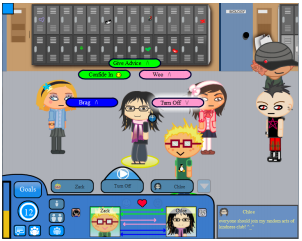
\includegraphics[scale=0.7]{Images/PromWeek.png}
\caption{A screenshot of \textit{Prom Week} showing the social interaction options available to the player. The HUD also shows the relationship between the player and the target player. [12]}
\end{figure}

For example, if the player has the goal of attaining a date to attend the prom with, they may try to use the ``flirt'' social interaction on another character. This may, or may not, succeed and the social state across both characters will be altered according to the author-specified rules that dictate the social norm of that interaction \textbf{(Figure 2)}. The results of this interaction are stored in a database of social facts, acting as a sort of global memory. CiF also incorporates `trigger rules' which ``encode the cascading effects of social state change'' outside of the current interaction [13]. Once an interaction has finished, these triggers are run over the social network in order to update the social state of each character.

The CiF system itself does not attempt to model the entire story world. It is a social reasoning component that aims to realistically model the rules and patterns that characters should follow during any social exchange. In contrast to Cavazza et al.'s hierarchical task network planning approach [11] (and other approaches such as behaviour trees), CiF encapsulates domain knowledge in one large rulebase that represents the social norms of a given story world. The system chooses each character's behaviour based on these rules. CiF doesn't create a static series of events, but the logic of the story world, the characters involved, and their goals. CiF is inherently driven by the simulation of social exchanges, therefore the way in which goals are met is entirely emergent and unplanned. This supports Aylett's initial description of emergent narratives as emerging from the interactions of characters, rather than being pre-planned [5][6].\\

\newline An extension of the CiF system [14] was proposed by Guimaraes et al. that adapted the social physics simulator to a first-person perspective, implemented as a publicly downloadable modification in the \textit{Elder Scrolls V: Skyrim} game engine. The results saw an extended interaction space for in-game NPCs leading to more believable characters and an improved player experience, as confirmed by the modification's popularity [15] and the results of user testing.

\subsubsection{Modelling Emotional Behaviour - FearNot! application and FAtiMA agent architecture}
Louchart et al. produced The \textit{FearNot!} (Fun with Empathic Agents Reaching Novel Outcomes in Teaching!) storytelling system, designed for anti-bullying education and inspired by Forum Theatre [3]. \textit{FearNot!} generates short episodes where a character is bullied and the victim asks the player for advice. The player's advice has an impact on the victim's emotional state which in turn influences the actions of that character in the next episode \textbf{(Figure 3)}. Each character is represented by an intelligent agent architecture which includes an ``affective appraisal system and autonomous action selection capabilities'' [3]. In addition to the character agents, an additional story facilitator agent is used for selecting characters, props, and locations for successive episodes. The story facilitator takes the player's actions and the characters' emotional state into consideration, generating an unscripted episode which is logically coherent to previously transpired events. For example, if the player ``has advised the character to hit back, it may set up an episode where victim and bully confront each other directly'' [3]. The story facilitator is comparable to \textit{Virtual Storyteller}'s ``virtual director'' [10] which stores global story data and uses it to influence and adapt the narrative. However, \textit{FearNot!}'s director does not perform global agent control and thus each agent remains fully autonomous. Rather than influencing characters directly, the director appraises past episodes and the current state of the story world and uses this data to generate logically cohesive succesive content.\\

\newline \textit{FearNot!} takes a focus on character-based emergent narratives which Louchart et al. explain requires a "bottom-up approach in which story elements are synthesised in real time via character interaction" [3]. This contrasts branching plot-based narratives which are created top-down with the story being comprised of fixed plot elements. In \textit{FearNot!'s} approach, characters are defined by their emotions, personalities, action tendencies, goals and emotional reactions. This is `organic' because characters will only perform actions in-character, according to their own personality and desires, rather than requiring global action management. From the author's point of view, developing a character requires the static checking of character actions (e.g. making sure all actions have reachable preconditions) and the simulation of interaction in various contexts to confirm that the character acts in-line with the author's vision.\\

\newline \textit{FearNot!} uses an affective agent architecture dubbed \textit{FAtiMA} (\textbf{F}earnot \textbf{A}ffec\textbf{TI}ve \textbf{M}ind \textbf{A}rchitecture) [19][20]. The architecture is designed to use author-specified emotions and personality to influence the behaviour of characters. It includes two essential components: a continuous planner (allowing characters to act intelligently and perform action repair and situated reasoning during unexpected events) and an emotional personality model (which effects the way characters react to events and provides a greater sense of believability). Appraisal is the assessment of any given event in relation to a character's emotions and influences their choice of actions towards their goals (world states they desire). \textit{FAtiMA} allows for the description of appraisal rules which define the event to be appraised and the desirability of the event on the target character [3]. Using this data, the character's emotions are updated. For example, an event in which a character is bullied would have very low desirability and produce negative emotions for the victim character.\\

\begin{figure}
\centering
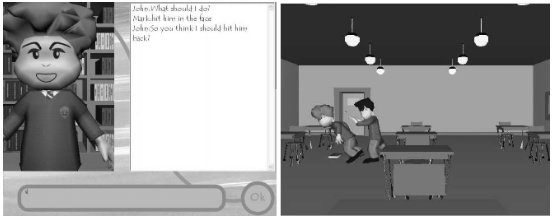
\includegraphics[scale=0.43]{Images/FearNot.png}
\caption{A screenshot of the \textit{FearNot!} system showing a scenario where a child is being bullied and asks the player for advice. [3]}
\end{figure}

\newline Emotions are a crucial aspect of the agent architecture and influence each character's planning process. Emotional values can be used as pre-conditions for potential actions. The use of emotional values (amongst other data such as memories and social relations) can be used by agents to perform rational processing to intelligently select actions that will help them towards their goal. However, \textit{FAtiMA} also incorporates non-cognitive reactional processing: "spontaneous reactions triggered by intense emotions [and] not part of the planning process" [3]. With this feature, characters with extreme emotional states can react with appropriate actions; for example, a character with extremely negative emotions may spontanenously burst out crying. This is an attempt to allow characters to react entirely emotionally to certain situations, rather than cognitively, and adds an extra layer of believability.

\textit{FAtiMA}'s planning system requires actions to be defined with preconditions (such as ranges of emotional values or certain event preconditions) and effects (the outcome of the action). Characters use actions to react to stimuli (other character's actions) or to help them achieve their goals. Goals can be defined as active pursuits or interests. Active pursuit goals are defined as world states which a character strives to attain whereas interest goals are world states that the character wants to maintain. Interest goals can help characters choose certain actions over others because actions which modify desired world states are considered undesirable [3].\\

\newline Due to \textit{FAtiMA}'s flexibility and modularity, some extensions to the architecture have been proposed in order to provide greater functionality and believability. Dias et al. successfully extended FAtiMA, allowing agents to ``explicitly talk about their internal thoughts and report their personal past experiences ... [using] a specific type of episodic long term memory'' [21][22]. This is a promising idea because memory is an important part of the human decision making process and helps add more believability to characters.

\subsection{Emergent Narrative in Commercial Games}
Emergent narrative generation methods are not solely practiced in research; many commercially successful games have yielded interesting and unique methods for generating unplanned interactive storylines:

\subsubsection{The Sims}
\textit{The Sims} [16] is possibly one of the most widely played and easily recognisable video games of the simulation genre and is a textbook example of emergent narrative creation. 
From the outset the player is provided with great freedom, being able to create their own character; namely their appearance, but later installments in the franchise allow for the selection of personality traits that help define unique characters and change the results of social interactions. This is interesting because it allows the player to be a partial director and their choices in the character creation stage will affect how their avatar acts and what stories emerge during the game. There is no rigid storyline to the game and no plot the player must follow. Instead, the user ``plays god'' and instructs their avatar to perform desired actions such as socialising with other characters or interacting with objects in the world. Typically, a narrative emerges from the results of the player's actions and the interactions of the player's avatar with other characters (e.g. neighbours or family members). For example, the player may choose to use the ``flirt'' social interaction with another character they meet in a bar who will respond accordingly. This could lead to an in-game relationship, marriage, and even starting a family, all of which involve a growing narrative. \textbf{(Figure 4)}.\\

\begin{figure}
\centering
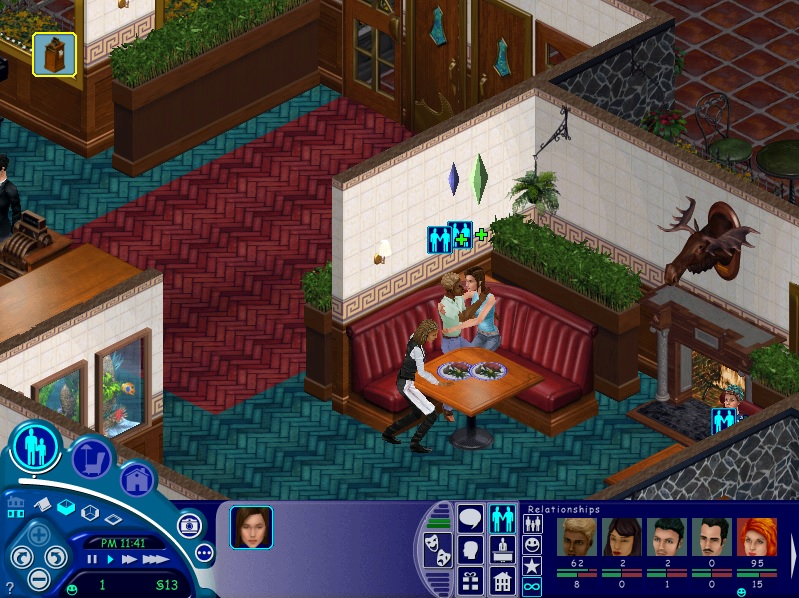
\includegraphics[scale=0.37]{Images/sims.png}
\caption{A screenshot of \textit{The Sims} showing two characters bonding in a restaurant. In the bottom-right corner, relationships between characters are displayed graphically. [16]}
\end{figure}

\newline \textit{The Sims} includes the simulation of personalities, emotions, needs, and social traits, not dissimilar to \textit{Prom Week}'s social AI system or the \textit{FAtiMA} agent architecture's emotional personality model. Characters can also have immediate responses to emotional state, alike the \textit{FearNot!} system's action tendencies. For example, if a character's mood is low enough they will ignore the player's actions in order to satisfy their own needs and improve their mood first.\\

\newline Despite the high level of freedom given to the player, a serious limitation of \textit{The Sims}' narrative generation is the fact that the quality of the story relies entirely on the player's choice of interesting actions. Should they desire, the player could allow their avatar to live in complete isolation and only watch TV all day, thus resulting in a lack of narrative entirely. There is no guarantee that engaging high-quality narratives will be produced because the player acts autocratically as spectator and director.

\begin{table*}[t]
\centering
\caption{Component Specification for Successful Emergent Narrative Systems}
    \begin{tabular}{| c | p{13cm} |}
    \hline
    Component & Rationale \\ \hline
    Emotional Personality Model & Emergent systems require a character-focused bottom-up approach to design. Modelling unique personalities and keeping track of emotions allows characters to react differently, yet believably, to each story event. This also includes the social relationships between each character. \\ \hline
    Continuous Planner & Characters need to be able to act on their emotions and react to occuring story events. A planning component allows characters to manage personal goals that they're working towards and construct a series of executable actions to reach that goal. The planner component should also exhibit situated reasoning (allowing characters to react believably to specific events, especially unanticipated ones) and action repair (allowing characters to adapt their plans should they experience action failure) [11]. \\ \hline
    Appraisal & Appraisal is the assessment of any given event in relation to a character's emotions and influences their choice of actions towards their goals (world states they desire). Appraisal is essential for each agent's decision making process. \\ \hline
    Memory / Knowledge Base & Characters need some way of remembering events that have transpired in the story. Memories of the positive and negative actions they have experienced should influence a character's decision making process. This could be a single global knowledge base that all agents can refer to (such as the \textit{Comme il Faut} system's global rulebase [13]), or encapsulated inside the agent architecture itself [21]. The former assumes perfect knowledge of the storyworld for each character, but the latter allows each character to have varying amounts of knowledge. \\ \hline
    (Optional) Virtual Director & Many systems use some form of virtual director; a seperate agent that uses general story-world knowledge about the plot structure to adapt and improve the story [3][10][17]. This shouldn't be used to perform global action control for individual agents (removing full agent autonomy), rather to facilitate the generation of interesting cohesive content (as in \textit{FearNot!} [3]) or to constantly analyse the state of the storyworld and create appropriate story events that challenge the player (as in Rimworld [17]). \\ \hline
    \end{tabular}
\end{table*}[t]

\subsubsection{RimWorld}
\textit{RimWorld} [17] is a ``colony simulator'' game that was inspired by the highly realistic simulation-based approach to game design pioneered by \textit{Dwarf Fortress} [18], a sandbox game which sees the player manage the livelihood of a group of dwarves.

\textit{RimWorld} tasks the player with managing a group of spaceship crash survivors as they construct a colony on their new home: an alien planet. The player must ``manage colonists' moods, needs, individual wounds, and illnesses'' [17]. The game is driven by an intelligent AI storyteller and its creator describes the game not as a strategy game, but as a story generator in its own right. At any given moment, the AI storyteller analyzes the colony's situation and decides which event will make the best story [17]. Accordingly, the AI storyteller can be considered \textit{RimWorld}'s equivalent of \textit{Virtual Storyteller}'s ``virtual director'' [10], or \textit{FearNot!'s} story facilitator;  a seperate agent that maintains story-world knowledge about the plot structure and uses it to adapt the narrative at run-time. As a result, \textit{RimWorld} suffers less of the narrative limitations experienced in \textit{The Sims} where the quality of the story relies wholly on how compelling a player's actions are. Because the AI storyteller acts as an agent itself, its goal can be considered the generation of a ``good'' story and its process of selecting suitable actions to change the narrative's course can be considered a form of action repair, ensuring that player actions that divert from its goal are eventually remedied. 

\begin{figure}
\centering
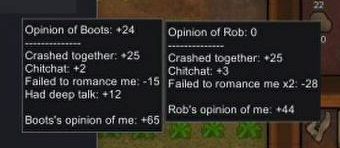
\includegraphics[scale=0.68]{Images/rimworld.png}
\caption{A screenshot of \textit{RimWorld} showing a comparison of the relationships between two characters. Recent events and their related numerical mood effects are shown. [17]}
\end{figure}

For example, players have the choice of upgrading the colony with weapons and defences to protect characters from periodic waves of attackers. The AI storyteller can evaluate the colony's level of defense and ensure that the next wave of attackers is strong enough to prove challenging to the player and therefore exciting enough to produce a ``good'' narrative.\\

\newline \textit{RimWorld} includes a sophisticated social simulation inspired by \textit{The Sims}. Colonists have traits which help them react in unique ways to social interactions (e.g. ``Night-Owl'' colonists have a better mood if they're up at night and ``Greedy'' colonists have a mood loss if their bedrooms aren't impressive) and emotions which change according to various stimuli \textbf{(Figure 5)}. Similar to the \textit{FearNot!} system [3], the state of these emotions determine which actions a character will take. Colonists can also reactively process emotions, identical to \textit{FearNot!}'s action tendencies. This manifests as a ``mental break'' where extreme mood values cause colonists to disregard player instructions entirely and engage in fully autonomous, usually obstructive, behaviour. For example, if a colonist's mood is low enough they may engage in an uncontrollable psychotic episode of pyromancy, igniting the colony's buildings.

Colonists have memories and can remember the effects of actions for varied lengths of time. For example, a recently divorced colonist may suffer a mood reduction for several months. Memories can influence the decision making process, allowing disgruntled colonists to react to those that have wronged them. Such reactions depend on the character's personality; for example, a character may choose to violently attack their aggressor with a weapon or simply insult them.

\section{Criteria for Successful Systems}
\noindent By evaluating existing emergent narrative systems and their components it is possible to establish a set of criteria that successful future systems should follow. We propose the component specification shown in \textbf{(Table 1)}.


\section{Designing a Hybrid System}
\subsection{Agent Architecture}
\subsubsection{Emotional Personality Model}
\subsubsection{Continuous Planning}
\subsection{Goals}
\subsubsection{Active Pursuit vs. Interest}
\subsubsection{Managing and Executing Actions}
\subsubsection{Action Priority Queueing}
\subsubsection{Need for Asynchronicity}
\subsection{Virtual Director}
\subsubsection{Potential for Genetic Algorithm}

\section{Implementation}
\subsection{Unity}
\subsection{Prototype System}
\subsection{Tools for Authors}

\section{Project Progress}
\subsection{Project Management}
\subsection{Contributions and Reflections}
\subsection{Moving Forward}

\addcontentsline{toc}{section}{References}

\begin{thebibliography}{20}

\bibitem{Bostan and Marsh}
Bostan B., \& Marsh T. (2012). 
``Fundamentals Of Interactive Storytelling''. 
\textit{Academic Journal of Information Technology}, \textbf{3}(8), pp. 20-42

\bibitem{Riedl}
Riedl M. O. (2010). 
``A Comparison of Interactive Narrative System Approaches using Human Improvisational Actors''.
\textit{Georgia Institute of Technology, College of Computing}

\bibitem{Authoring Emergent Games}
Louchart S., Aylett R., Kriegel M., Dias J., Figueiredo R., \& Paiva A. (2008).
``Authoring Emergent Narrative-Based Games''.
\textit{Journal of Game Development}, \textbf{3}(1), pp. 19-37

\bibitem{Solving the Narrative Paradox in VEs}
Louchart S., \& Aylett R. (2003).
``Solving the Narrative Paradox in VEs - Lessons from RPGs''.
\textit{In: Rist T., Aylett R.S., Ballin D., Rickel J. (eds) Intelligent Virtual Agents. IVA 2003. Lecture Notes in Computer Science, Vol. 2792}, pp. 244-248

\bibitem{EmergentNarrative}
Aylett R. (2000).
``Emergent Narrative, Social Immersion and ``Storification''''.
\textit{Proceedings Narrative and Learning Environments Conference}, Edinburgh, Scotland

\bibitem{Towards Emergent Narrative}
Aylett R. (1999).
``Narrative in Virtual Environment - Towards Emergent Narrative''.
\textit{In: Proceedings of the AAAI Fall Symposium on Narrative Intelligence, 1999}

\bibitem{Massively Collaborative Authoring}
Kriegel M., \& Aylett R. (2008).
``Emergent Narrative As A Novel Framework For Massively Collaborative Authoring''.
\textit{In: Prendinger H., Lester J., Ishizuka M. (eds) Intelligent Virtual Agents. IVA 2008. Lecture Notes in Computer Science, vol 5208}

\bibitem{Novel Writer}
Klein S., Aeschlimann J.F., Balsiger D.F., Converse S.L., Court C., Foster M., Lao R., Oakley J.D., \& Smith J. (1973).
``Automatic Novel Writing: A Status Report''.
\textit{University of Wisconsin}

\bibitem{Tale-Spin}
Meehan, J.R. (1977).
``Tale-Spin, an Interactive Program that Writes Stories''.
\textit{In: Proceedings of the Fifth International Joint Conference on Artificial Intelligence (IJCAI)}

\bibitem{The Virtual Storyteller}
Theune, M., Faas S., Nijholt, A., \& Heylen, D. (2003).
``The Virtual Storyteller: Story Creation by Intelligent Agents''.
\textit{In: Proceedings of TIDSE 2003: Technologies for Interactive Digital Storytelling and Entertainment}

\bibitem{Character-based Interactive Storytelling}
Cavazza, M., Charles, F., \& Mead, S.J. (2002).
``Character-based Interactive Storytelling''.
\textit{IEEE Intelligent Systems}, \textbf{17}(4), pp.17-24

\bibitem{Prom Week}
McCoy, J., Treanor, M., Samuel, B., Reed, A., Mateas, M., \& Wardrip-Fruin, N. (2013).
``Prom Week: Designing past the game/story dilemma''.
\textit{In: Proceedings of the Eighth International Conference on the Foundations of Digital Games (FDG 2013)}, pp.94-101

\bibitem{CiF}
McCoy, J., Treanor, M., Samuel, B., Wardrip-Fruin, N., \& Mateas, M (2013).
``Comme il Faut: A System for Authoring Playable Social Models''.
\textit{In: Proceedings of the Seventh AAAI Conference on Artificial Intelligence and Interactive Digital Entertainment}, pp.158-163

\bibitem{CiF-CK}
Guimaraes, M., Santos, P., \& Jhala, A. (2017).
``CiF-CK: An Architecture for Social NPCs in Commercial Games''.
\textit{2017 IEEE Conference on Computational Intelligence and Games (CIG)}, pp.126-123

\bibitem{CiF-CK Mod Page}
Social NPCs Mod for Elder Scrolls V: Skyrim, available at: https://www.nexusmods.com/skyrim/mods/77792/ [Accessed 21 Nov. 2018]

\bibitem{The Sims}
Maxis: The Sims. Electronic Arts (2000)

\bibitem{RimWorld}
Tynan Sylvester: RimWorld. Ludeon Studios (2018), available at: https://rimworldgame.com/ [Accessed 21 Nov. 2018]

\bibitem{Dwarf Fortress}
Adams, T., Adams, Z.: Slaves to Armok: God of Blood Chapter II: Dwarf Fortress (2006)

\bibitem{FAtiMA}
Dias, J., Macscarenhas, S., \& Paiva, A. (2014)
``FAtiMA Modular: Towards an Agent Architecture with
a Generic Appraisal Framework''.
\textit{Emotion Modeling} pp.44-56

\bibitem{Emotional Agents}
Dias, J., \& Paiva, A. (2005)
``Feeling and Reasoning: A Computational Model for Emotional Agents''.
\textit{In: Proceedings of 12th Portuguese Conference on Artificial Intelligence, EPIA 2005,} pp.127-140

\bibitem{FAtiMA with Memory}
Dias, J., W. C. Ho., Vogt, T., Beeckman, N., Paiva1, A., \& Andre, E. (2007)
"I Know What I Did Last Summer: Autobiographic Memory in Synthetic Characters".
\textit{Affective Computing and Intelligent Interaction: Second International Conference, ACII 2007 Lisbon, Portugal, September 12-14, 2007 Proceedings} pp.606-617

\bibitem{Autobiographical Memory}
Ho, W.C. \& Watson, S. (2006) 
"Autobiographic Knowledge for Believable Virtual Characters".
\textit{In: Proceedings of Intelligent Virtual Agents 2006 (IVA 2006)} pp.383-394

\bibitem{Virtual Theatre}
Hayes-Roth, B., Brownston, L., \& Sincoff, E. (1995)
"Directed Improvisation by Computer Characters".
\textit{Technical Report KSL 95-04, Knowledge Systems Laboratory, Stanford University, 1995}

\bibitem{Improv System}
Perlin, K., \& Goldberg, A.
"Improv: A System for Scripting Interactive Actors in Virtual Worlds".
\textit{In: Proceedings of the 23rd Annual Conference on Computer Graphics and Interactive Techniques (SIGGRAPH '96) pp.205-216 }




\end{thebibliography}
 
\end{document}
